\section{Analysis (AN)}
\subsection{Änderungsmaße}
\begin{minipage}{0.45\textwidth}
    \subsubsection{absolute Änderung}
        Die absolute Änderung von $f$ zwischen $a$ und $b$ ist der Betrag der Differenz der Funktionswerte:
        \begin{equation}
            Delta f = f(b) - f(a)
        \end{equation}
    \subsubsection{relative Änderung}
        Die relative Änderung von $f$ zwischen $a$ und $b$ ist die absolute Änderung im Verhältnis zum Anfangswert:
        \begin{equation}
            \frac{\Delta f}{f(a)} = \frac{f(b) - f(a)}{f(a)}
        \end{equation}
\end{minipage}
\hfill
\begin{minipage}{0.5\textwidth}
    \centering 
    \begin{tikzpicture}
        \begin{axis}[
            xmin=-0.2, xmax=4,
            ymin=-0.2,   ymax=3,
            xtick={0.42628, 3.16444},
            ytick={0.58433, 1.98469},
            xticklabels = {$a$, $b$},
            yticklabels = {$f(a)$, $f(b)$},
            axis lines=middle,
            xlabel={$x$},
            ylabel={$y$},
            samples=200,
            width=8cm,
            height=6cm,
            axis line style={latex-latex},
        ]
        % f(x)
        \addplot[accent, very thick, domain=0:3.8] {x^4/6 - 4*x^3/3 + 10*x^2/3 - 13*x/6 + 1}
            node[pos=0.6, above left] {$f(x)$};
        
        % Punkte
        \def\xa{0.42628}
        \def\ya{0.58433}
        \def\xb{3.16444}
        \def\yb{1.98469}
        
        % gestrichelte Hilfslinien für Punkt A
        \draw[densely dashed, black]
          (axis cs:\xa,0) -- (axis cs:\xa,\ya);
        \draw[densely dashed, black]
          (axis cs:0,\ya) -- (axis cs:\xb,\ya);
        
        % gestrichelte Hilfslinien für Punkt B
        \draw[densely dashed, black]
          (axis cs:\xb,0) -- (axis cs:\xb,\ya);
        \draw[densely dashed, black]
          (axis cs:0,\yb) -- (axis cs:\xb,\yb);
        
        % Punkte markieren
        \addplot[only marks, mark=*, mark size=2pt, black]
          coordinates {( \xa, \ya ) ( \xb, \yb )};
        
        % Steigungsdreieck
        \draw[<->, thick, black]
          (axis cs:\xb,\ya) -- (axis cs:\xb,\yb)
            node[midway, right] {$\Delta y$};
        \end{axis}
    \end{tikzpicture}
\end{minipage}
\\[20pt]
\noindent
\begin{minipage}{0.45\textwidth}   
    \subsubsection{mittlere Änderungsrate}
        Die mittlere Änderungsrate/Sekantensteigung oder auch Differenzenquotient von $f$ zwischen $a$ und $b$ ist die Differenz der Funktionswerte geteilt durch die Differenz der Argumente:
        \begin{equation}
            \frac{\Delta y}{\Delta x} = \frac{f(b) - f(a)}{b - a} = k
        \end{equation}
\end{minipage}
\hfill
\begin{minipage}{0.5\textwidth}
    \centering 
    \begin{tikzpicture}
        \begin{axis}[
            xmin=-0.2, xmax=4,
            ymin=-0.2,   ymax=3,
            xtick={0.42628, 3.16444},
            ytick={0.58433, 1.98469},
            xticklabels = {$a$, $b$},
            yticklabels = {$f(a)$, $f(b)$},
            axis lines=middle,
            xlabel={$x$},
            ylabel={$y$},
            samples=200,
            width=8cm,
            height=5cm,
            axis line style={latex-latex},
        ]
        % f(x)
        \addplot[accent, very thick, domain=0:3.8] {x^4/6 - 4*x^3/3 + 10*x^2/3 - 13*x/6 + 1}
            node[pos=0.6, above left] {$f(x)$};
        
        % Punkte
        \def\xa{0.42628}
        \def\ya{0.58433}
        \def\xb{3.16444}
        \def\yb{1.98469}
        
        % gestrichelte Hilfslinien für Punkt A
        \draw[densely dashed, black]
          (axis cs:\xa,0) -- (axis cs:\xa,\ya);
        \draw[densely dashed, black]
          (axis cs:0,\ya) -- (axis cs:\xa,\ya);
        
        % gestrichelte Hilfslinien für Punkt B
        \draw[densely dashed, black]
          (axis cs:\xb,0) -- (axis cs:\xb,\ya);
        \draw[densely dashed, black]
          (axis cs:0,\yb) -- (axis cs:\xb,\yb);
        
        % Punkte markieren
        \addplot[only marks, mark=*, mark size=2pt, black]
          coordinates {( \xa, \ya ) ( \xb, \yb )};
        
        % Sekante durch die beiden Punkte
        \addplot[black, thick, domain=-0.2:4]
          {( \yb-\ya )/( \xb-\xa )*(x-\xa) + \ya};
        
        % Steigungsdreieck
        \draw[thick, black]
          (axis cs:\xa,\ya) -- (axis cs:\xb,\ya)
            node[midway, below] {$\Delta x$};
        \draw[thick, black]
          (axis cs:\xb,\ya) -- (axis cs:\xb,\yb)
            node[midway, right] {$\Delta y$};
        \end{axis}
    \end{tikzpicture}
\end{minipage}
\\[20pt]
\noindent
\begin{minipage}{0.45\textwidth}
    \subsubsection{momentane Änderungsrate}
    Die momentane Änderungsrate/Tangentensteigung oder auch Differentialquotient von $f$ an der Stelle $x_0$ ist die Ableitung von $f$ an dieser Stelle:
    \begin{align}
        f'(x_0) &= \left.\frac{df}{dx}\right|_{x = x_0} = \frac{df}{dx}(x_0) \\
        &= \lim_{b \to a} \frac{f(b) - f(a)}{b - a} \nonumber \\
        &= \lim_{\Delta x \to x_0} \frac{f(x+\Delta x)-f(x)}{\Delta x} \nonumber
    \end{align}
\end{minipage}
\hfill
\begin{minipage}{0.5\textwidth}
    \centering 
    \begin{tikzpicture}
        \begin{axis}[
            xmin=-0.2, xmax=4,
            ymin=-0.2, ymax=3,
            xtick={1.7},
            ytick={1.79135},
            xticklabels = {$x_0$},
            yticklabels = {$y_0$},
            axis lines=middle,
            xlabel={$x$},
            ylabel={$y$},
            samples=200,
            width=8cm,
            height=5cm,
            axis line style={latex-latex},
        ]
        % f(x)
        \addplot[accent, very thick, domain=0:3.8]
          {x^4/6 - 4*x^3/3 + 10*x^2/3 - 13*x/6 + 1}
          node[pos=0.8, above] {$f(x)$};
    
        % Werte
        \def\xnull{1.7}
        \def\ynull{1.79135}    % f(1.7)
        \def\m{0.882}          % f'(1.7)
    
        % Tangente in x0: y = m*(x - x0) + y0
        \addplot[black, thick, domain=0.8:2.6]
          {\m*(x-\xnull) + \ynull};
    
        % Punkt (x0, y0)
        \addplot[only marks, mark=*, mark size=2pt, black]
          coordinates {(\xnull, \ynull)};
    
        % Hilfslinien zu den Achsen für (x0, y0)
        \draw[densely dashed, black]
          (axis cs:\xnull,0) -- (axis cs:\xnull,\ynull);
        \draw[densely dashed, black]
          (axis cs:0,\ynull) -- (axis cs:\xnull,\ynull);
    
        \def\dx{0.5}
        
        % Punkte des Steigungsdreiecks berechnen
        \pgfmathsetmacro{\xB}{\xnull + \dx}      % x-Koordinate des rechten Punktes
        \pgfmathsetmacro{\yB}{\ynull}           % gleiche Höhe wie y0
        \pgfmathsetmacro{\yC}{\ynull + \m*\dx}  % y0 + m * Δx
        
        % Steigungsdreieck zeichnen
        \draw[thick, black]
          (axis cs:\xnull,\ynull) -- (axis cs:\xB,\yB)
            node[midway, below] {$\Delta x$};
        \draw[thick, black]
          (axis cs:\xB,\yB) -- (axis cs:\xB,\yC)
            node[midway, right] {$\Delta y$};
    
        \end{axis}
    \end{tikzpicture}
\end{minipage}
\vspace{20pt}
\\
Der Differenzenquotient liefert also die Steigung der Sekante durch zwei Punkte des Graphen. Wenn man nun die zwei Punkte immer weiter zusammenführt (der Abstand $\Delta x$ geht gegen 0) erhält man den Differentialquotient (die Tangentensteigung). Der Differentialquotient ist als die Ableitung $f'(x)$ definiert und liefert die Steigung der Funktion an einem Punkt.

\subsection{Regeln für das Differenzieren}
Berechnet man allgemein die Ableitung einer Funktion $f(x)$ so erhält man wieder eine Funktion $f'(x)$ welche die Steigung von $f$ in jedem Punkt beschreibt. Die entsprechende Ableitungsfunktion kann mithilfe der Ableitungsregeln und/oder Tabellen gefunden werden.
\subsubsection{Ableitungsregeln}
\begin{align}
    &\text{Faktorregel}     && (k \cdot f)' = k \cdot f' \\[8pt]
    &\text{Summenregel}     && (f \pm g)' = f' \pm g' \\[8pt]
    &\text{Produktregel}    && (f \cdot g)' = f' \cdot g + f \cdot g' \\[8pt]
    &\text{Quotientenregel} && \left(\frac{f}{g}\right)' =
        \frac{f' \cdot g - f \cdot g'}{g^2} \quad \text{für } g(x) \neq 0 \\[8pt]
    &\text{Kettenregel}     && h(x) = f(g(x)) \Rightarrow
        h'(x) = f'(g(x)) \cdot g'(x)
&\end{align}
\\
In folgender Tabelle sind alle gängigen Funktionen und deren Ableitungen und Integrale dargestellt. Diese Tabelle befindet sich in der Formelsammlung der Matura. \\[5pt]
\begin{center}
\begin{tabular}{lll}
\textbf{Funktion} & \textbf{Ableitungsfunktion} & \textbf{Stammfunktion} \\
\hline\\[-8pt]  % nur hier zusätzlicher Abstand
$f(x) = k$ 
  & $f'(x) = 0$ 
  & $F(x) = k \cdot x$ \\[4pt]

$f(x) = x^{q}$ 
  & $f'(x) = q \cdot x^{q-1}$ 
  & $F(x) = \dfrac{x^{q+1}}{q+1} \quad \text{für } q \neq -1$ \\[4pt]

 &  & $F(x) = \ln(|x|) \quad \text{für } q = -1$ \\[4pt]

$f(x) = e^{x}$ 
  & $f'(x) = e^{x}$ 
  & $F(x) = e^{x}$ \\[4pt]

$f(x) = a^{x}$ 
  & $f'(x) = \ln(a)\cdot a^{x}$ 
  & $F(x) = \dfrac{a^{x}}{\ln(a)}$ \\[4pt]

$f(x) = \ln(x)$ 
  & $f'(x) = \dfrac{1}{x}$ 
  & $F(x) = x\cdot \ln(x) - x$ \\[4pt]

$f(x) = \log_{a}(x)$ 
  & $f'(x) = \dfrac{1}{x\cdot \ln(a)}$ 
  & $F(x) = \dfrac{1}{\ln(a)}\cdot (x\cdot \ln(x) - x)$ \\[4pt]

$f(x) = \sin(x)$ 
  & $f'(x) = \cos(x)$ 
  & $F(x) = -\cos(x)$ \\[4pt]

$f(x) = \cos(x)$ 
  & $f'(x) = -\sin(x)$ 
  & $F(x) = \sin(x)$ \\[4pt]

$f(x) = \tan(x)$ 
  & $f'(x) = 1 + \tan^{2}(x) = \dfrac{1}{\cos^{2}(x)}$ 
  & $F(x) = -\ln(|\cos(x)|)$ \\[4pt]

$g(x) = k \cdot f(x)$ 
  & $g'(x) = k \cdot f'(x)$ 
  & $G(x) = k \cdot F(x)$ \\[4pt]

$h(x) = f(x) \pm g(x)$ 
  & $h'(x) = f'(x) \pm g'(x)$ 
  & $H(x) = F(x) \pm G(x)$ \\[4pt]

$g(x) = f(k \cdot x)$ 
  & $g'(x) = k \cdot f'(k \cdot x)$ 
  & $G(x) = \dfrac{1}{k}\cdot F(k \cdot x)$ \\
\end{tabular}
\end{center}
\vspace{10pt}
\noindent
Eine besonders wichtige Eigenschaft ist, dass sich die Exponentialfunktion ($e^x$) sowohl beim Ableiten als auch beim Integrieren nicht verändert.

\pagebreak
\subsection{Ableitungsfunktion, Stammfunktion}
\subsubsection{Das Integrieren als Umkehrung des Differenzierens}
Das ermitteln der Stammfunktion $F(x)$ ist die Umkehrung des \emph{Differenzierens} und wird als \emph{Integrieren} bezeichnet.
\begin{center}
    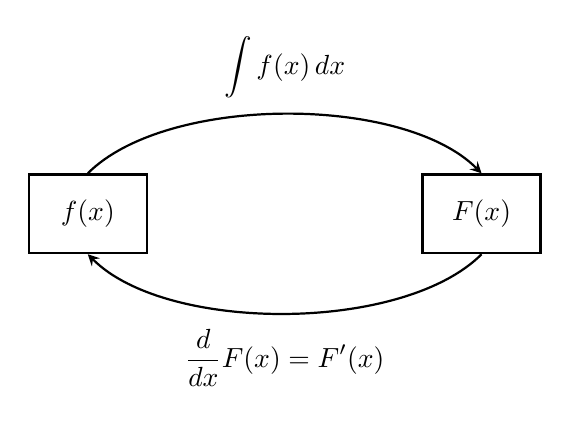
\begin{tikzpicture}[>=stealth]
    \node[draw, thick, rectangle, minimum width=1.5cm, minimum height=1cm, align=center]  
        (left)  at (0,0) {$f(x)$};  
    \node[draw, thick, rectangle, minimum width=1.5cm, minimum height=1cm, align=center]  
        (right) at (5,0) {$F(x)$};
      
    \draw[thick,->]  
      (left.north) .. controls +(1,1) and +(-1,1) .. (right.north)  
      node[midway, above, yshift=2pt] {$\displaystyle \int f(x)\,dx$};  
      
    \draw[thick,<-]    
      (left.south) .. controls +(1,-1) and +(-1,-1) .. (right.south)   
      node[midway, below, yshift=-2pt]    
      {$\displaystyle \frac{d}{dx}F(x) = F'(x)$};
    \end{tikzpicture}
\end{center}
\subsubsection{Unbestimmtes Integral}
Ist eine Funktion $F(x)$ eine Stammfunktion von $f(x)$, so sind auch alle Funktionen
\begin{equation}
    F(x)+C,\quad C\in \mathrm{R}
\end{equation}
Stammfunktionen von $f(x)$. \\
Die Menge aller Stammfunktionen wird als \textbf{unbestimmtes Integral} von $f(x)$ bezeichnet und man schreibt:
\begin{equation}
    \int f(x)\,dx = F(x) + C
\end{equation}
Das unbestimmte Integral kann durch Anwendung von Regeln und/oder Tabellen ermittelt werden.
\\[20pt]

\subsubsection{Kurvendiskussion}
\begin{minipage}{0.45\textwidth}
{
    \centering
    \textbf{Funktion durch Punkte} \\
}
{
    Geht eine Funktion durch einen Punkt $P(P_x,P_y)$ so erhält man folgende Gleichung:
    \begin{equation*}
        f(P_x) = P_y
    \end{equation*}
}
{
    \centering
    \begin{tikzpicture}
      \begin{axis}[
        width=7cm, height=5cm,
        axis lines=middle,
        xmin=-0.2, xmax=2,
        ymin=-0.2, ymax=1.5,
        xlabel={$x$}, ylabel={$y$},
        xtick={0,1}, xticklabels={0,$P_x$},
        ytick={0,1}, yticklabels={0,$P_y$},
        domain=0:1.75,
      ]
        \addplot[accent, ultra thick] {-0.9*x^3+1.7*x^2-0.3*x+0.5}
            node[pos=0.2, above=2pt] {$f(x)$};
        \addplot[only marks, mark=*, mark size=2pt, black] coordinates {(1,1)};
        \node[below right, black] at (axis cs:1,1) {P};
        \draw[densely dashed] (axis cs:0,1) -- (axis cs:1,1);
        \draw[densely dashed] (axis cs:1,0) -- (axis cs:1,1);
      \end{axis}
    \end{tikzpicture}
}\\[0.5em]
\end{minipage}
\hfill
\begin{minipage}{0.45\textwidth}
{
    \centering
    \textbf{Nullstellen} \\
}
{
    Hat eine Funktion an einer Position eine Nullstelle erhält man folgende Gleichung:
    \begin{equation*}
        f(x_0) = 0
    \end{equation*}
}
{
    \centering
    \begin{tikzpicture}
      \begin{axis}[
        width=7cm, height=5cm,
        axis lines=middle,
        xmin=-0.2, xmax=3,
        ymin=-1, ymax=1,
        xlabel={$x$}, ylabel={$y$},
        xtick={0,1,2}, xticklabels={0,$ $, $\;\,x_0$}, 
        ytick={-0.5,0.5}, yticklabels={},
        domain=0:2.3,
      ]
        \addplot[accent, ultra thick] {0.4*x^3-0.7*x^2-0.15*x-0.1}
            node[pos=0.2, below=2pt] {$f(x)$};
        \addplot[only marks, mark=*, mark size=2pt, black] coordinates {(2,0)};
        \node[above left, black] at (axis cs:2,0) {N};
      \end{axis}
    \end{tikzpicture}
}\\[0.5em]
\end{minipage}

\noindent
\begin{minipage}{0.45\textwidth}
{
    \centering
    \textbf{Extrempunkte} \\
}
{
    Hat eine Funktion einen Extrempunkt so ist die erste Ableitung null:
    \begin{equation*}
        f'(x_0)=0
    \end{equation*}
}
{
    \centering
      \begin{tikzpicture}
        \begin{axis}[
            width=7cm, height=5cm,
            axis lines=middle,
            xmin=-0.2, xmax=2.5,
            ymin=-0.2, ymax=2,
            xlabel={$x$}, ylabel={$y$},
            xtick={0,1,2}, xticklabels={0,$x_0$, $ $}, 
            ytick={0,0.5,1.5}, yticklabels={},
            domain=0:2.2,
        ]
            \addplot[accent, ultra thick] {-0.9*x^2+1.8*x+0.6}
                node[pos=0.7, right=3pt] {$f(x)$};
            \addplot[only marks, mark=*, mark size=2pt, black] coordinates {(1,1.5)};
            \node[above, black] at (axis cs:1,1.5) {Max};
            \draw[densely dashed] (axis cs:1,0) -- (axis cs:1,1.5);
            \end{axis}
            \end{tikzpicture}
}\\[0.5em]
\end{minipage}
\hfill
\begin{minipage}{0.45\textwidth}
{
    \centering
    \textbf{Wendepunkte} \\
}
{
    Hat eine Funktion einen Wendepunkt so ist die zweite Ableitung null:
    \begin{equation*}
        f''(x_0)=0
    \end{equation*}
}
{
    \centering
    \begin{tikzpicture}
      \begin{axis}[
        width=7cm, height=5cm,
        axis lines=middle,
        xmin=-0.5, xmax=2,
        ymin=-0.2, ymax=2,
        xlabel={$x$}, ylabel={$y$},
        xtick={0,0.5,1,1.5}, xticklabels={0,$x_0$, $ $,$ $}, 
        ytick={0,0.5,1.5}, yticklabels={},
        domain=-0.4:1.7,
      ]
        \addplot[accent, ultra thick] {-1.4*x^3+2.1*x^2+0.5*x+0.6}
            node[pos=0.7, right=3pt] {$f(x)$};
        \addplot[only marks, mark=*, mark size=2pt, black] coordinates {(0.5,1.2)};
        \node[above left, black] at (axis cs:0.5,1.2) {WP};
        \draw[densely dashed] (axis cs:0.5,0) -- (axis cs:0.5,1.2);
      \end{axis}
    \end{tikzpicture}
}\\[0.5em]
\end{minipage}
\begin{minipage}{0.45\textwidth}
{
    \centering
    \textbf{Steigung an einem Punkt} \\
}
{
    Hat eine Funktion einen Extrempunkt so ist die erste Ableitung null:
    \begin{equation*}
        f'(x_0) = \frac{\Delta y}{\Delta x} = k
    \end{equation*}
}
{
    \centering
    \begin{tikzpicture}
      \begin{axis}[
        width=7cm, height=5cm,
        axis lines=middle,
        xmin=-0.2, xmax=2,
        ymin=-0.2, ymax=1.5,
        xlabel={$x$}, ylabel={$y$},
        xtick={0,1}, xticklabels={0,$x_0$},
        ytick={0,1}, yticklabels={},
        domain=0:1.75,
      ]
        \addplot[accent, ultra thick] {-0.9*x^3+1.7*x^2-0.3*x+0.5}
            node[pos=0.2, below=2pt] {$f(x)$};
        \addplot[black, very thick, domain=0.3:1.8] {0.4*x+0.6};
        \addplot[only marks, mark=*, mark size=2pt, black] coordinates {(1,1)};
        \draw[densely dashed] (axis cs:1,0) -- (axis cs:1,1);
        \draw[] (axis cs:1,1) -- (axis cs:1.5,1)
            node[midway, below, black] at (axis cs:1,1) {$\Delta x$};
        \draw[] (axis cs:1.5,1) -- (axis cs:1.5,1.2)
            node[midway, right, black] at (axis cs:1,1) {$\Delta y$};
      \end{axis}
    \end{tikzpicture}
}\\[0.5em]
\end{minipage}
\hfill
\begin{minipage}{0.45\textwidth}
{
    \centering
    \textbf{Steigungswinkel} \\
}
{
    Hat eine Funktion einen Wendepunkt so ist die zweite Ableitung null:
    \begin{equation*}
        \tan{(\alpha)} = \frac{\Delta y}{\Delta x} = f'(x_0)
    \end{equation*}
}
{
    \centering
    \begin{tikzpicture}
      \begin{axis}[
        width=7cm, height=5cm,
        axis lines=middle,
        xmin=0.5, xmax=1.8,
        ymin=0.7, ymax=1.3,
        xlabel={$x$}, ylabel={$y$},
        xtick={0,1}, xticklabels={0,$x_0$},
        ytick={0,1}, yticklabels={},
        domain=0:1.5,
      ]
        \addplot[accent, ultra thick] {-0.9*x^3+1.7*x^2-0.3*x+0.5}
            node[pos=0.2, below=2pt] {$f(x)$};
        \addplot[black, very thick, domain=0.3:1.8] {0.4*x+0.6};
        \addplot[only marks, mark=*, mark size=2pt, black] coordinates {(1,1)};
        \draw[densely dashed] (axis cs:1,0) -- (axis cs:1,1);
        \draw[] (axis cs:1,1) -- (axis cs:1.5,1)
            node[midway, below, black] at (axis cs:1,1) {$\Delta x$};
        \draw[] (axis cs:1.5,1) -- (axis cs:1.5,1.2)
            node[midway, right, black] at (axis cs:1,1) {$\Delta y$};
        \node at (axis cs:1.2,1.03) {$\alpha$};
      \end{axis}
    \end{tikzpicture}
}\\[0.5em]
\end{minipage}
\begin{minipage}{0.45\textwidth}
{
    \centering
    \textbf{Monotonie} \\
}
{
    Das Monotonieverhalten hängt mit der ersten Ableitung zusammen:
    \begin{align*}
        \text{sms: } f'(x)>0,  \quad \text{ms: } f'(x) \geq 0 \\
        \text{smf: } f'(x)<0,  \quad \text{mf: } f'(x) \leq 0 
    \end{align*}
}
{
    \centering
      \begin{tikzpicture}
        \begin{axis}[
            width=7cm, height=5cm,
            axis lines=middle,
            xmin=-0.2, xmax=2.5,
            ymin=-0.2, ymax=2,
            xlabel={$x$}, ylabel={$y$},
            xtick={0,1,2}, xticklabels={}, 
            ytick={0,0.5,1.5}, yticklabels={},
            domain=0:2.2,
        ]
            \addplot[accent, ultra thick] {-0.9*x^2+1.8*x+0.6}
                node[pos=0.7, right=3pt] {$f(x)$};
            \draw[densely dashed] (axis cs:1,0) -- (axis cs:1,2);
            \node[above, black] at (axis cs:0.5,0.4) {$f'(x)>0$};
            \node[above, black] at (axis cs:1.5,0.4) {$f'(x)<0$};
            \end{axis}
        \end{tikzpicture}
}\\[0.5em]
\end{minipage}
\hfill
\begin{minipage}{0.45\textwidth}
{
    \centering
    \textbf{Krümmung} \\
}
{
    Das Krümmungsverhalten hängt mit der zweiten Ableitung zusammen:
    \begin{align*}
        \text{links/pos. gekrümmt/konvex: } f''(x) > 0 \\
        \text{rechts/neg. gekrümmt/konkav: }  f''(x) < 0  
    \end{align*}
}
{
    \centering
    \begin{tikzpicture}
      \begin{axis}[
        width=7cm, height=5cm,
        axis lines=middle,
        xmin=-1, xmax=2,
        ymin=-0.2, ymax=2,
        xlabel={$x$}, ylabel={$y$},
        xtick={-.5,0,0.5,1,1.5}, xticklabels={},
        ytick={0,0.5,1.5}, yticklabels={},
        domain=-0.7:1.7,
      ]
        \addplot[accent, ultra thick] {-1.4*x^3+2.1*x^2+0.5*x+0.6}
            node[pos=0.7, right=6pt] {$f(x)$};
        \addplot[only marks, mark=*, mark size=2pt, black] coordinates {(0.5,1.2)};
        \draw[densely dashed] (axis cs:0.5,0) -- (axis cs:0.5,2);
        \node[above, black] at (axis cs:-0.1,1.2) {$f''(x)>0$};
        \node[above, black] at (axis cs:1,0.8) {$f''(x)<0$};
      \end{axis}
    \end{tikzpicture}
}\\[0.5em]
\end{minipage}
\\

\subsubsection{Umkehraufgaben}
Zu den Eigenschaften von Funktionen gibt es sehr viele Aufgaben. Gesucht ist meist eine Polynomfunktion $n$-ten Grades.
Man verwendet hierfür den Ansatz:
\[
    f(x) = a_0 x^0 + a_1 x^1 + a_2 x^2 + \dots + a_n x^n
\]
Zusätzlich sind dann immer Bedingungen gegeben welche die gesuchte Funktion erfüllen muss. Aus diesen Bedingungen kann man dann Gleichungen Formen bis man ein Gleichungssystem erhält. Wichtig ist, dass man für jede Unbekannte eine Gleichung braucht (es werden $n$ unabhängige Gleichungen benötigt).
Das fertige Gleichungssystem kann dann mit Geogebra gelöst werden.
\\[20pt]


\begin{aufgabe}
    Eine Solarzelle wandelt kurzwellige Strahlungsenergie, wie zum Beispiel Sonnenlicht, direkt in elektrische Energie um.
    In der nachstehenden Grafik ist die Leistungskurve einer Solarzelle dargestellt:
    \begin{center}
    \begin{tikzpicture}
        \begin{axis}[
        width=15cm, height=8cm,
        axis lines=middle,
        xmin=-2, xmax=45,
        ymin=-10, ymax=150,
        xlabel={Spannung in V}, ylabel={Leistung in W},
        xtick={0,2,4,6,8,10,12,14,16,18,20,22,24,26,28,30,32,34,36,38,40,42,44},
        ytick={0,20,40,60,80,100,120,140},
        grid=both,
        ]
        \addplot[accent, ultra thick, domain=20:40] {-0.002*x^4+0.19*x^3-6.9*x^2+117*x-680}
            node[pos=0.7, above right] {$f(x)$};
        \addplot[black, ultra thick, domain=0:20] {5*x}
            node[pos=0.7, above left] {$g(x)$};
            
        \addplot[only marks, mark=*, mark size=2pt, black]
          coordinates {(20,100)}
          node[above=2pt] {$A$};
        
        \addplot[only marks, mark=*, mark size=2pt, black]
          coordinates {(30,130)}
          node[above=2pt] {$B$};
        
        \end{axis}
    \end{tikzpicture}
    \end{center}
    Der Verlauf der Leistungskurve wird im Intervall $[0; 20]$ durch eine lineare Funktion $g$ und
    im Intervall $[20; 40]$ durch eine Polynomfunktion $f$ vom Grad 4 beschrieben. Im Punkt $A$
    gehen die beiden Funktionsgraphen knickfrei ineinander über (das bedeutet, dass die
    Funktionen an der Stelle den gleichen Funktionswert und die gleiche Steigung haben). Im
    Punkt $B$ hat die Funktion $f$ einen Hochpunkt. Die maximale Leistung der Solarzelle beträgt
    130 Watt. 
    \[
        f(x) = a \cdot x^4 + b \cdot x^3 + c \cdot x^2 + d \cdot x + e
    \]
    $x$ \dots Spannung in Volt \\
    $f(x)$ \dots Leistung der Spannung $x$ in Watt \\[10pt]
    Stellen sie ein Gleichungssystem auf, mit dem die Koeffizienten $a,b,c,d$ und $e$ berechnet werden können.
\end{aufgabe}
\begin{loesung} \\
    Die einfachsten Gleichungen erhalten wir aus den Punkte $A$ und $B$:
    \begin{align*}
        f(20)=100 \\
        f(30)=130
    \end{align*}
    Bei der Spannung $x=40\,\mathrm{V}$ ist eine Nullstelle:
    \[ 
        f(40)=0
    \]
    Bei der Spannung $x=30\,\mathrm{V}$ ist ein Maximum:
    \[
        f'(30)=0
    \]
    Die Funktion $f(x)$ hat im Punkt $A$ dieselbe Steigung wie $g(x)$. Die Steigung von $g(x)$ kann man über das Steigungsdreieck ablesen.
    \[
        f'(20) = g'(20) = 5
    \]
    Das Gleichungssystem kann mit Geogebra gelöst werden.
    \begin{geogebracode}
        f(x):=a*x^4+b*x^3+c*x^2+d*x+e // CAS: Wichtig: := nach f(x) setzen
        f(20)=100
        f(30)=100
        f(40)=0
        f'(30)=0
        f'(20)=5
        // Gleichungen auswählen -> Löse oder NLöse
    \end{geogebracode}
    
\end{loesung}

\pagebreak
\subsubsection{Graphisches Differenzieren \& Integrieren}
Es wurde bereits festgestellt, dass die Ableitung die Tangentensteigung einer Funktion an jedem Punkt beschreibt. Möchte man nun graphisch die Ableitung herausfinden, ist es praktisch, gewisse Punkte zu verwenden.
\begin{center}
\begin{tikzpicture}
  %%%%%%%%%%%%% 1. Plot: F(x) %%%%%%%%%%%%%
  \begin{axis}[
    width=0.8\textwidth,
    height=0.4\textwidth,
    axis lines=middle,
    xmin=-1.7, xmax=2.7,   % Bereich etwas nach rechts verschoben
    ymin=-1.4, ymax=4.4,
    samples=200,
    xlabel={$x$}, ylabel={$y$},
    xtick={-1.5,-0.5,0.5,1.5,2.5},
    ytick={-1,0,1,2,3,4},
    xticklabels ={},
    domain=-1.5:2.5,
    name=topplot,
    axis line style={latex-latex},
  ]
    \addplot[accent, ultra thick] {(x-0.5)^3 - 3*(x-0.5) + 1}
        node[pos=0.9, left] {$f(x)$};

    \addplot[only marks, mark=*, mark size=2pt, black] coordinates {(-0.5,3)};
    \node[above left, black] at (axis cs:-0.5,3) {Max};
    \coordinate (Pmax) at (axis cs:-0.5,3);

    \addplot[only marks, mark=*, mark size=2pt, black] coordinates {(1.5,-1)};
    \node[above=2pt, black] at (axis cs:1.5,-1) {Min};
    \coordinate (Pmin) at (axis cs:1.5,-1);

    \addplot[only marks, mark=*, mark size=2pt, black] coordinates {(0.5,1)};
    \node[above right, black] at (axis cs:0.5,1) {WP};
    \coordinate (Pwp) at (axis cs:0.5,1);
  \end{axis}

  %%%%%%%%%%%%% 2. Plot: f(x) = F'(x) %%%%%%%%%%%%%
  \begin{axis}[
    at={(topplot.south west)},
    anchor=north west,
    yshift=-1cm,
    width=0.8\textwidth,
    height=0.4\textwidth,
    axis lines=middle,
    xmin=-1.7, xmax=2.7,
    ymin=-4.4, ymax=1.4,
    samples=200,
    xlabel={$x$}, ylabel={$y'$},
    xtick={-1.5,-0.5,0.5,1.5,2.5},
    ytick={-4,-3,-2,-1,0,1},
    domain=-1.5:2.5,
    name=middleplot,
    axis line style={latex-latex},  
  ]
    \addplot[accent, ultra thick] {3*(x-0.5)^2 - 3}
        node[pos=0.58, below right] {$f'(x)$};

    % Nullstellen von f
    \addplot[only marks, mark=*, mark size=2pt, black] coordinates {(-0.5,0) (1.5,0)};
    \node[above right, black] at (axis cs:-0.5,0) {NS};
    \node[above left, black] at (axis cs:1.5,0) {NS};
    \coordinate (Dleft)  at (axis cs:-0.5,0);
    \coordinate (Dright) at (axis cs:1.5,0);

    % Minimum von f
    \addplot[only marks, mark=*, mark size=2pt] coordinates {(0.5,-3)};
    \node[below] at (axis cs:0.5,-3) {Min};
    \coordinate (Dmin) at (axis cs:0.5,-3);
  \end{axis}

  %%%%%%%%%%%%% 3. Plot: f'(x) = F''(x) %%%%%%%%%%%%%
  \begin{axis}[
    at={(middleplot.south west)},
    anchor=north west,
    yshift=-1cm,
    width=0.8\textwidth,
    height=0.4\textwidth,
    axis lines=middle,
    xmin=-1.7, xmax=2.7,
    ymin=-7, ymax=7,
    samples=200,
    xlabel={$x$}, ylabel={$y''$},
    xtick={-1.5,-0.5,0.5,1.5,2.5},
    ytick={-6,-4,-2,0,2,4,6},
    domain=-1.5:2.5,
    name=bottomplot,
    axis line style={latex-latex},  
  ]
    % f'(x) = 6(x-0.5)
    \addplot[accent, ultra thick] {6*(x-0.5)}
        node[pos=0.85, above right] {$f''(x)$};

    % Nullstelle von f' bei x = 0.5
    \addplot[only marks, mark=*, mark size=2pt, black] coordinates {(0.5,0)};
    \node[above right, black] at (axis cs:0.5,0) {NS};
    \coordinate (DprimeNS) at (axis cs:0.5,0);
  \end{axis}

  %%%%%%%%%%%%% Verbindungen zwischen den Plots %%%%%%%%%%%%%
  % F-Max <-> Nullstelle von f links
  \draw[densely dashed] (Pmax) -- (Dleft);
  % F-Min <-> Nullstelle von f rechts
  \draw[densely dashed] (Pmin) -- (Dright);
  % Wendepunkt von F <-> Minimum von f
  \draw[densely dashed] (Pwp) -- (Dmin);
  % Minimum von f <-> Nullstelle von f'
  \draw[densely dashed] (Dmin) -- (DprimeNS);

\end{tikzpicture}
\end{center}
Man kann erkennen:
\begin{itemize}
    \item Wendepunkte werden zu Extrempunkten
    \item Extrempunkte werden zu Nullstellen
    \item Ist $f(x)$ monoton steigend, so ist $f'(x)>0$
    \item Ist $f(x)$ monoton fallend, so ist $f'(x)<0$
    \item Ist $f(x)$ rechtsgekrümmt so ist $f''(x)<0$
    \item Ist $f(x)$ linksgekrümmt so ist $f''(x)>0$
\end{itemize}

\subsection{Summation und Integral}
\subsubsection{Ober- und Untersummen}
Um den Flächeninhalt unter Funktionen zu approximieren (annähern) können Ober- bzw. Untersummen verwendet werden. Der Bereich unter der Kurve wird dabei in Rechtecke unterteilt -- je feiner die Zerlegung, desto genauer die Annäherung.
\\
Hier soll der Flächeninhalt zwischen der Funktion $f(x)$ und der $x$-Achse im Intervall $[a,b]$ berechnet werden. Der Bereich wird in $n$ Rechtecke unterteilt. Die Breite eines Rechtecks berechnet sich wie folgt: 
\begin{equation}
    \Delta x = \frac{b-a}{n}
\end{equation}
\\
\noindent

\pgfmathsetmacro{\a}{1}
\pgfmathsetmacro{\b}{5}
\pgfmathsetmacro{\n}{12}
\pgfmathsetmacro{\h}{(\b-\a)/\n} % = 1/3

\begin{minipage}{0.45\textwidth}  
\textbf{Obersumme}\\[10pt]
{
    \centering  
    \begin{tikzpicture}[color=black,/pgf/declare function={f(\x)=-\x^4/4 + (8*\x^3)/3 - (37*\x^2)/4 + (71*\x)/6 - 1;}]
        \begin{axis}[  
            width = 7cm, height=6cm,  
            domain=0.5:5.5,  
            samples=200,  
            axis lines=middle,  
            xlabel={$x$},  
            ylabel={$f(x)$},  
            xtick={\a,\b},  
            xticklabels={a,b},  
            ymin=0,ymax=6.5,  
            xmin=0.5,xmax=6,  
        ]  
          
        \addplot [ultra thick, black] {f(x)};  
          
        \addplot[  
            ybar interval,  
            draw=black,  
            fill=accent,  
            fill opacity=0.1,  
            bar width=\h,  
        ]  
        coordinates {  
            (\a         , 4.01050)  
            (\a+\h      , 3.86420)  
            (\a+2*\h    , 3.44444)  
            (\a+3*\h    , 3.00000)  
            (\a+4*\h    , 2.71605)  
            (\a+5*\h    , 3.00000)  
            (\a+6*\h    , 3.56790)  
            (\a+7*\h    , 4.29630)  
            (\a+8*\h    , 5.00000)  
            (\a+9*\h    , 5.41975)  
            (\a+10*\h   , 5.44294)  
            (\a+11*\h   , 5.22222)  
            (\b         , 0)  
        };  
        \end{axis}  
    \end{tikzpicture}  
}
\\
Es wird in jedem Intervall die Funktionsstelle mit dem größten Funktionswert genommen. Die Summe aller Rechtecke ergibt die Obersumme $O_n$, welche als obere Schranke für den tatsächlichen Flächeninhalt gilt.
\begin{equation}
    O_n = \sum_{i=1}^n \sup_{x_{i-1}<x<x_i} \Delta x \quad \footnotemark
\end{equation}
\end{minipage}  
\footnotetext{Das Supremum ist die kleinste obere Schranke}
\hfill  
\begin{minipage}{0.45\textwidth}  
\textbf{Untersumme}\\[10pt]
{
    \centering  
    \begin{tikzpicture}[color=black,/pgf/declare function={f(\x)=-\x^4/4 + (8*\x^3)/3 - (37*\x^2)/4 + (71*\x)/6 - 1;}]
        \begin{axis}[  
            width = 7cm, height=6cm,  
            domain=0:5.5,  
            samples=200,  
            axis lines=middle,  
            xlabel={$x$},  
            ylabel={$f(x)$},  
            ymin=0,ymax=6.5,  
            xmin=0.5,xmax=6,  
            xtick={\a,\b},  
            xticklabels={a,b},  
        ]  
          
        \addplot [ultra thick] {f(x)};  
          
        \addplot[  
            ybar interval,  
            draw=black,  
            fill=accent,  
            fill opacity=0.1,  
            bar width=\h,  
        ]  
        coordinates {  
            (\a         , 3.86420)  
            (\a+\h      , 3.44444)  
            (\a+2*\h    , 3.00000)  
            (\a+3*\h    , 2.71605)  
            (\a+4*\h    , 2.67156)  
            (\a+5*\h    , 2.70370)  
            (\a+6*\h    , 3.00000)  
            (\a+7*\h    , 3.56790)  
            (\a+8*\h    , 4.29630)  
            (\a+9*\h    , 5.00000)  
            (\a+10*\h   , 5.22222)  
            (\a+11*\h   , 4.00000)  
            (\b         , 0)  
        };  
        \end{axis}  
    \end{tikzpicture}  
}
\\
Es wird in jedem Intervall die Funktionsstelle mit dem kleinsten Funktionswert genommen. Die Summe aller Rechtecke ergibt die Untersumme $U_n$, welche als untere Schranke für den tatsächlichen Flächeninhalt gilt.
\begin{equation}
    U_n = \sum_{i=1}^n \inf_{x_{i-1}<x<x_i} \Delta x \quad \footnotemark
\end{equation}
\end{minipage}
\footnotetext{Das Infimum ist die größte untere Schranke}

\vspace{20pt}
\noindent
Eine wichtige Eigenschaft ist
\begin{equation}
    U_n \leq A \leq O_n
\end{equation}
Macht man die Zerlegung unendlich klein, so erhält man als Grenzwert das \emph{Unbestimmte Integral} der Fläche. Das $dx$ beschreibt das infinitesimal klein werdende $\Delta x$.
\begin{equation}
\int_a^b f(x)\,dx = 
    \lim_{n \rightarrow \infty}O_n= 
    \lim_{n \rightarrow \infty}U_n
\end{equation}

\begin{aufgabe}
    Gegeben sei die Funktion $f(x) = -0.2x^2 + 0.8x + 2$ \\
    Berechne die Untersumme $U_n$ sowie die Obersumme $O_n$ im Intervall $[-1,3]$ für $n=5$ Zerlegungen. Vergleiche die Ergebnisse mit dem tatsächlichen Wert des Flächeninhalts.
\end{aufgabe}
\vfill

\begin{loesung}
    Zuerst berechnen wir die Breite der Rechtecke: 
    \begin{equation*}
        \Delta x = \frac{b-a}{n} = \frac{4-(-1)}{5} = 1
    \end{equation*}
    Um herauszufinden welche Funktionswerte für die Ober- und Untersumme verwendet werden stellen wir die Funktion graphisch dar.
        \begin{center}
    \begin{tikzpicture}
        \begin{axis}[
            width=8cm, height=6cm,
            axis lines=middle,
            xmin=-2.5, xmax=5,
            ymin=-0.2, ymax=2.5,
            xlabel={$x$}, ylabel={$y$},
            xtick={-1,0,1,2,3,4},
            ytick={0,1,2}, yticklabels={},
            domain=-2:4.5,
            axis line style={latex-latex},
            title=Untersumme,
        ]
            \addplot[accent, ultra thick, samples=200] {-0.2*x^2+0.8*x+1.2};
                %node[pos=0.85, above right] {$f(x)$};

             \addplot[  
                ybar interval,  
                draw=black,  
                fill=accent,  
                fill opacity=0.1,  
                bar width=1,  
            ]  
            coordinates {  
                (-1,0.2)  
                (0,1.2)
                (1,1.8)
                (2,1.8) 
                (3,1.2)
                (4,1.2)
            };  

                \addplot[only marks, mark=*, mark size=2pt]
                    coordinates {  
                    (-1,0.2)  
                    (0,1.2)
                    (1,1.8)
                    (3,1.8) 
                    (4,1.2)
                };  
            \node[above left] at (axis cs:-1,0.2) {\small$f(-1)$};
            \node[above left] at (axis cs:0,1.2) {\small$f(0)$};
            \node[above=2pt] at (axis cs:1,1.8) {\small$f(1)$};
            \node[above=2pt] at (axis cs:3,1.8) {\small$f(3)$};
            \node[above right] at (axis cs:4,1.2) {\small$f(4)$};

            \end{axis}
    \end{tikzpicture}
    \hspace{25pt}
    \begin{tikzpicture}
    \begin{axis}[
            width=8cm, height=6cm,
            axis lines=middle,
            xmin=-2.5, xmax=5,
            ymin=-0.2, ymax=2.5,
            xlabel={$x$}, ylabel={$y$},
            xtick={-1,0,1,2,3,4},
            ytick={0,1,2}, yticklabels={},
            domain=-2:4.5,
            axis line style={latex-latex},
            title=Obersumme,
        ]
        \addplot[accent, ultra thick, samples=200] {-0.2*x^2+0.8*x+1.2};
            %node[pos=0.85, above right] {$f(x)$};

         \addplot[  
            ybar interval,  
            draw=black,  
            fill=accent,  
            fill opacity=0.1,  
            bar width=1,  
        ]  
        coordinates {  
            (-1,1.2)  
            (0,1.8)
            (1,2.0)
            (2,2.0) 
            (3,1.8)
            (4,1.2)
        };  

            \addplot[only marks, mark=*, mark size=2pt]
                coordinates {  
                (0,1.2)  
                (1,1.8)
                (2,2.0)
                (3,1.8)
            };  
        \node[above left] at (axis cs:0,1.2) {\small$f(0)$};
        \node[above left] at (axis cs:1,1.8) {\small$f(1)$};
        \node[above=2pt] at (axis cs:2,2) {\small$f(2)$};
        \node[above right] at (axis cs:3,1.8) {\small$f(3)$};

        \end{axis}
    \end{tikzpicture}
    \end{center}
    Für die Untesumme nehmen wir immer den niedrigsten Wert in einem Abschnitt, für die Obersumme immer den Höchsten.
    \begin{equation*}
        U_n = f(-1) \cdot \Delta x + f(0) \cdot \Delta x +f (1) \cdot \Delta x + f(3) \cdot \Delta x + f(4) \cdot \Delta x = 6.2
    \end{equation*}
    \begin{equation*}
        O_n = f(0) \cdot \Delta x + f(1) \cdot \Delta x + f(2) \cdot \Delta x + f(2) \cdot \Delta x + f(3) \cdot \Delta x = 8.8
    \end{equation*}
    Der tatsächliche Wert der Fläche ist:
    \begin{equation*}
        A = \int_{-1}^4 f(x) \, dx = 7.67
    \end{equation*}
    Es gilt also wie erwartet:
    \begin{equation*}
        U_n = 6.2 \;\leq\; A \;\leq\; 8.8 = O_n
    \end{equation*}
\end{loesung}

\subsubsection{Bestimmtes Integral}
Der Zusammenhang zwischen dem unbestimmten Integral und dem bestimmten Integral ist durch den \emph{Hauptsatz der Differential- und Integralrechnung} definiert.
\begin{equation}
    \int_a^b f(x)\,dx = F(x) \big|_a^b = F(b)-F(a)
\end{equation}

\begin{bsp}
\begin{align*}
    &\int_{-2}^2 x^3-4x \, dx = \left .\frac{1}{4} x^4 - \frac{1}{2}2x^2 \right|_{-2}^{2} \\[5pt]
    &= \left( \frac{1}{4} 2^4 - \frac{1}{2}2\cdot 2^2 \right) - \left( \frac{1}{4} (-2)^4 - \frac{1}{2}2\cdot(-2)^2 \right) = 0
\end{align*}
\end{bsp}
\noindent
Das Ergebnis des Integrals liefert den Wert null, was am Anfang etwas komisch erscheint.
Es ist jedoch wichtig zu wissen, dass das unbestimmte Integral die \emph{orientierte Fläche} zwischen einer Funktion und der $x$-Achse berechnet. Das heißt Flächen unter der $x$-Achse werden negativ gewertet. \\
Eine weitere wichtige Eigenschaft ist, dass sich beim Vertauschen der Integrationsgrenzen das Vorzeichen ändert.
\begin{equation}
    \int_a^b f(x)\,dx = -\int_b^a f(x)\,dx 
\end{equation}

\begin{bsp}
    Betrachten wir die Funktion $f(x)=x^3-4x$ etwas genauer. Jetzt möchten wir die absolute Fläche zwischen der Funktion und der $x$-Achse berechnen.
    \begin{center}
    \begin{tikzpicture}
        \begin{axis}[
            width=12cm, height=8cm,
            axis lines=middle,
            xmin=-3, xmax=3,
            ymin=-4, ymax=4,
            xlabel={$x$}, ylabel={$y$},
            xtick={-2,-1,0,1,2},
            ytick={-3, -1, 0, 1, 3},
            domain=-2.8:2.8,
            axis line style={latex-latex},
        ]
            \addplot[accent, ultra thick, samples=200] {x^3-4*x}
                node[pos=0.7, above left] {$f(x)$};

            \node[black] at (axis cs:-1,1) {$A_1$};
            \node[black] at (axis cs:1,-1) {$A_2$};
            
            \end{axis}
    \end{tikzpicture}
    \end{center}
    Die einfachste Möglichkeit ist es einfach den Betrag der Funktion zu nehmen:
    \begin{align*}
        A = \int_{-2}^2 \left| f(x) \right| \, dx
    \end{align*}
    Ohne den Betrag müssen wir das Integral aber aufteilen.
    \begin{align*}
        A = A_1 + A_2 = \int_{-2}^0 f(x)\,dx + (-1)\cdot\int_0^2 f(x)\,dx
    \end{align*}
    Alternativ können wir auch die Grenzen des zweiten Integrals vertauschen:
    \begin{align*}
        A = \int_{-2}^0 f(x)\,dx + \int_2^0 f(x)\,dx
    \end{align*}
    Man kann auch das Betragssymbol verwenden:
      \begin{align*}
        A &= \int_{-2}^0 f(x)\,dx + \left| \int_0^2 f(x)\,dx \right| = \\
          &= \int_{-2}^0 f(x)\,dx + \int_0^2 \left| f(x) \right| \,dx
    \end{align*}
\end{bsp}

\subsubsection{Fläche zwischen zwei Funktionen}
Möchte man die Fläche zwischen zwei Funktionen im Intervall $[a,b]$ berechnen und die Funktion $f(x)$ liegt im ganzen Intervall über der Funktion $g(x)$ so berechnet sich die Fläche als:
\begin{equation}
    A = \int_a^b f(x)-g(x) \, dx = - \int_a^b g(x) - f(x) \, dx
\end{equation}
Weiß man nicht welche Funktion über welcher liegt kann man folgende Formel verwenden:
\begin{equation}
    A = \int_a^b \left| f(x)-g(x) \right| \, dx = 
        \int_a^b \left| g(x)-f(x) \right| \, dx
\end{equation}

\begin{bsp}
    In folgendem Beispiel möchten wir die Fläche zwischen den beiden Funktion $f(x)$ und $g(x)$ berechnen.
    \begin{center}
    \begin{tikzpicture}
        \begin{axis}[
            width=12cm, height=8cm,
            axis lines=middle,
            xmin=-3, xmax=2.5,
            ymin=-0.2, ymax=3,
            xlabel={$x$}, ylabel={$y$},
            xtick={-1.93,-0.5,0,1.33}, xticklabels={a,b,0,c},
            ytick={0,1,2},
            domain=-2.5:1.9,
            axis line style={latex-latex},
        ]
            \addplot[accent, ultra thick, samples=200] {0.8*x^3+0.5*x^2-1.7*x+0.9}
                node[pos=0.85, left] {$f(x)$};
            \addplot[accent2, ultra thick, samples=200] {-0.3*x^3-0.7*x^2+0.8*x+2.3}
                node[pos=0.85, left] {$g(x)$};

            \addplot[only marks, mark=*, mark size=2pt] coordinates {(-1.93,0.29)};
            \addplot[only marks, mark=*, mark size=2pt] coordinates {(-0.50,1.78)};
            \addplot[only marks, mark=*, mark size=2pt] coordinates {(+1.33,1.41)};

            \node[black] at (axis cs:-1.1,1.5) {$A_1$};
            \node[black] at (axis cs:0.6,1.5) {$A_2$};
            
            \end{axis}
    \end{tikzpicture}
    \end{center}
    Wir können unsere Formel mit dem Betrag anwenden:
    \begin{equation*}
        A = \int_a^c \left| f(x)-g(x) \right| \, dx
    \end{equation*}
    Wenn wir jedoch nicht den Betrag verwenden, müssen wir das Intervall zerlegen:
    \begin{align*}
        A = A_1 + A_2 = \int_a^b f(x) - g(x) \, dx + \int_b^c g(x) - f(x) \, dx
    \end{align*}
    Alternative Schreibweisen wären
    \begin{align*}
        A &= \int_a^b f(x) - g(x) \, dx + \int_b^c g(x) - f(x) \, dx \\
        &= \int_a^b f(x) - g(x) \, dx - \int_b^c f(x)-g(x) \, dx  && \text{($f,g$ und Vorzeichen vertauscht)}\\
        &= \int_a^b f(x) - g(x) \, dx + \left|\int_b^c f(x)-g(x) \, dx \right| && \text{($f,g$ vertauscht und Betrag)}\\
        &= \int_a^b f(x) - g(x) \, dx + \int_c^b f(x)-g(x) \, dx && \text{($f,g$ und Grenzen vertauscht)}
    \end{align*}
\end{bsp}